% Coverage--tightness frontier: our upper-bound predictor vs. leakage-safe
% baseline predictors, evaluated on the identical 2217 stage suffixes
% (12MP tier, normal capture, 12 sessions).
%
% GENERATED FILE -- do not edit values by hand. Source:
% evaluation-table_8U_12MP_normal_SEIP-review-metrics.xlsx,
% sheet "Baseline Comparison":
%   x = MeanRelativeSlackPct (mean positive headroom of the predicted upper
%       bound over the observed duration; lower = tighter bound),
%   y = StageCoveragePct (share of suffixes whose observed duration stayed
%       within the bound; higher = safer).
% Baselines are leave-one-session-out (LOSO) quantile predictors at target
% coverage 90/95/99% (markers left to right). "Ours (deployed)" is the
% production model's native operating point; "ours + residual calibration"
% adds a LOSO per-stage residual quantile on top of our bound.
%
% Requires: \usepackage{pgfplots} \pgfplotsset{compat=1.17}

\begin{figure}[t]
  \centering
  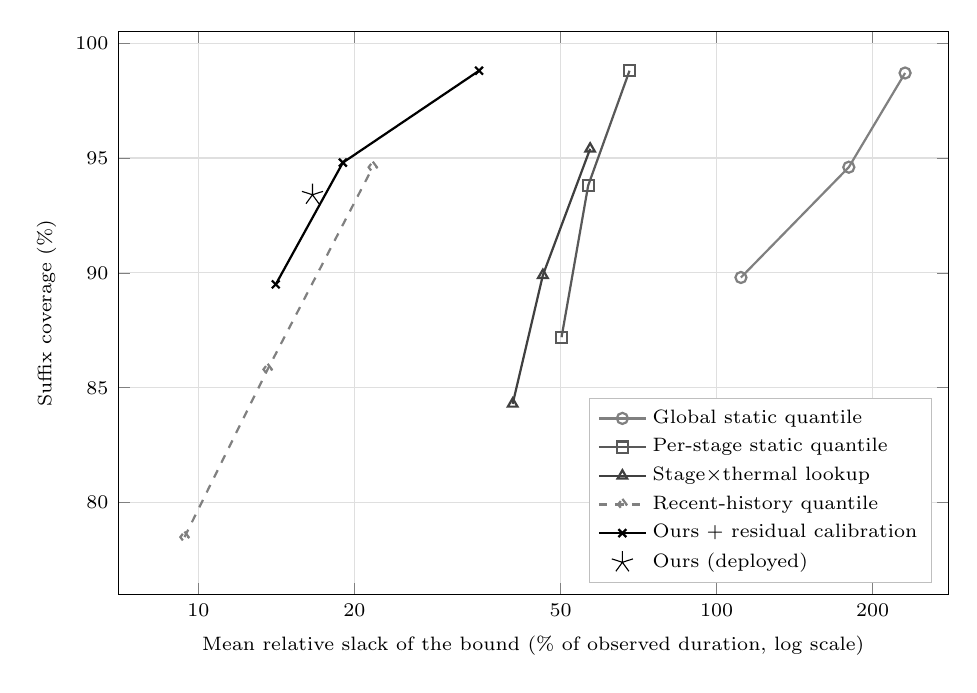
\begin{tikzpicture}
    \begin{axis}[
      width=\columnwidth,
      height=0.72\columnwidth,
      xmode=log,
      log ticks with fixed point,
      xtick={10,20,50,100,200},
      xlabel={Mean relative slack of the bound (\% of observed duration, log scale)},
      ylabel={Suffix coverage (\%)},
      xmin=7, xmax=280,
      ymin=76, ymax=100.5,
      grid=major,
      grid style={draw=gray!25},
      tick label style={font=\scriptsize},
      label style={font=\scriptsize},
      legend style={font=\scriptsize, at={(0.98,0.02)}, anchor=south east, draw=gray!50},
      legend cell align={left}
    ]
      \addplot[color=gray, mark=o, thick] coordinates {(111.4,89.8) (179.9,94.6) (231.0,98.7)};
      \addlegendentry{Global static quantile}
      \addplot[color=gray!70!black, mark=square, thick] coordinates {(50.2,87.2) (56.5,93.8) (67.9,98.8)};
      \addlegendentry{Per-stage static quantile}
      \addplot[color=gray!50!black, mark=triangle, thick] coordinates {(40.4,84.3) (46.2,89.9) (57.0,95.4)};
      \addlegendentry{Stage$\times$thermal lookup}
      \addplot[color=gray, mark=diamond, thick, dashed] coordinates {(9.4,78.5) (13.6,85.8) (21.7,94.6)};
      \addlegendentry{Recent-history quantile}
      \addplot[color=black, mark=x, thick] coordinates {(14.1,89.5) (19.0,94.8) (34.8,98.8)};
      \addlegendentry{Ours + residual calibration}
      \addplot[color=black, mark=star, only marks, mark size=4] coordinates {(16.6,93.4)};
      \addlegendentry{Ours (deployed)}
    \end{axis}
  \end{tikzpicture}
  \caption{Coverage--tightness trade-off of upper-bound predictors over the identical 2217 evaluated stage suffixes (12MP tier, normal capture, 12 burst sessions). Each baseline is a leakage-safe leave-one-session-out quantile predictor shown at target coverage 90/95/99\,\% (markers left to right); up and to the left is better (safer bounds that waste less budget, admitting more optional stages). At every matched coverage level, our predictor requires 1.6--9.5$\times$ less slack than the static and lookup baselines. The only baseline of comparable tightness, the recent-history quantile, reaches at most 94.6\,\% coverage at 21.7\,\% slack and is dominated there by our residual-calibrated variant (94.8\,\% at 19.0\,\%); its tighter operating points fall below 86\,\% coverage, which no timeout-averse controller can accept. All methods are evaluated on the same admitted, fully observed suffixes recorded under the deployed policy.}
  \label{fig:eval_frontier}
\end{figure}
